\documentclass[a4paper,12pt,fleqn]{article}%fleqn pour aligner les equations à gauche
\usepackage{../../Styles/Eval}


\newcommand{\chnum}{Chapitre 01}
\newcommand{\chtitle}{Identification d'espèces chimiques}
\newcommand{\dtype}{DS3}


\usepackage{hyperref} %cases à remplir informatiquement
\usepackage{multirow}
\begin{document}
\maketitle

\section{Mélanges ?}
On retrouve plusieurs flacons dans un ancien placard d'une pharmacie. Ces flacons contiennent des substances liquides dont on ignore la nature. On retrouve une vieille liste des produits stockés où figurent les informations suivantes : \\ solution saline : $\rho$ = \SI{1,01}{\gram\per\liter} ;\\ eau déminéralisée : $\rho$ = \SI{1,00}{\gram\per\liter} ;\\ éthanol : : $\rho$ = \SI{0,78}{\gram\per\liter} ;\\ acétone = : $\rho$ = \SI{0,79}{\gram\per\liter} ;\\ éther = : $\rho$ = \SI{0,71}{\gram\per\liter}
\begin{enumerate}
	\item Proposer un protocole permettant de déterminer la masse volumique d'une solution en utilisant du matériel de laboratoire courant. \textbf{(1pt)}
\end{enumerate}
	\fbox{\begin{minipage}{.9\textwidth}
	\begin{Form}
	\TextField[width = 17cm, height = 4.5cm,multiline,bordercolor=white]{}
	\end{Form}
	\end{minipage}}
	\fbox{\begin{minipage}{.05\textwidth}
	\vspace{4.5cm}
	\hspace{.5cm}
	\end{minipage}}

On met en place le protocole et on obtient le tableau de résultats suivant :

\begin{table}[h!]
	\begin{tabular}{|>{\centering}m{3.2cm}|>{\centering}m{3.2cm}|>{\centering}m{3.2cm}|>{\centering}m{3.2cm}|>{\centering\arraybackslash}m{3.2cm}|} \hline
	\textbf{Substance} & A & B & C & D \\ \hline
	$\mathbf{\rho}$ (\unit{\gram\per\milli\liter}) & 1,02 & 0,789 & 1,01 & 0,792 \\ \hline
	\end{tabular}
\end{table}
\begin{enumerate}[resume]
	\item Proposer, à partir des données, les identifications possibles pour chacune de ces substances. \textbf{(1pt)}
\end{enumerate}
	\fbox{\begin{minipage}{.90\textwidth}
	\begin{Form}
	\TextField[width = 17cm, height = 3cm,multiline,bordercolor=white]{}
	\end{Form}
	\end{minipage}}
	\fbox{\begin{minipage}{.05\textwidth}
	\vspace{3cm}
	\hspace{.5cm}
	\end{minipage}}
\begin{enumerate}[resume]
	\item Expliquer les limites de cette méthode. \textbf{(1pt)}
\end{enumerate}
	\fbox{\begin{minipage}{.9\textwidth}
	\begin{Form}
	\TextField[width = 17cm, height = 3cm,multiline,bordercolor=white]{}
	\end{Form}
	\end{minipage}}
	\fbox{\begin{minipage}{.05\textwidth}
	\vspace{3cm}
	\hspace{.5cm}
	\end{minipage}}

\newpage
Afin de déterminer plus finement la composition de ces trois échantillons, on propose de réaliser des tests d'identification d'ions.
\begin{enumerate}[resume]
	\item Proposer un schéma type de test à réaliser \textbf{(1pt)}
\end{enumerate}
	\fbox{\begin{minipage}{.9\textwidth}
	\begin{Form}
	\TextField[width = 17cm, height = 4cm,multiline,bordercolor=white]{}
	\end{Form}
	\end{minipage}}
	\fbox{\begin{minipage}{.05\textwidth}
	\vspace{4cm}
	\hspace{.5cm}
	\end{minipage}}
\begin{enumerate}[resume]
	\item Le résultat de ces tests sont indiqués dans la tableau ci-dessous. Proposer une identification définitive pour les échantillons en complétant la dernière ligne du tableau. \textbf{(1pt)}
\end{enumerate}
\begin{table}[h!]
	\begin{tabular}{|>{\centering}m{3.2cm}|>{\centering}m{3.2cm}|>{\centering}m{3.2cm}|>{\centering}m{3.2cm}|>{\centering\arraybackslash}m{3.2cm}|} \hline
	Substance & A & B & C & D \\ \hline
	Nitrate d'argent (\textit{présence d'ions \ce{Cl-}}) & $+$ & $-$ & $-$ & $-$ \\ \hline
	Permanganate de potassium (\textit{présence d'éthanol}) & $-$ & $-$ & $-$ & $+$ \\ \hline
	Sulfate de cuivre anhydre & $+$ & $-$ & $+$ & $-$ \\ \hline
	\textbf{Identification} & \begin{Form}
	\TextField[width = 3.2cm, height = 2cm,multiline,bordercolor=white]{}
	\end{Form}&\begin{Form}
	\TextField[width = 3.2cm, height = 2cm,multiline,bordercolor=white]{}
	\end{Form} &\begin{Form}
	\TextField[width = 3.2cm, height = 2cm,multiline,bordercolor=white]{}
	\end{Form} & \begin{Form}
	\TextField[width = 3.2cm, height = 2cm,multiline,bordercolor=white]{} 
	\end{Form}\\ \hline
	\end{tabular}
\end{table}
\begin{enumerate}[resume]
	\item Définir les notions de "corps pur" et de "mélange" puis préciser quelles substances sont des corps purs et lesquelles sont des mélanges. \textbf{(2pt)}
\end{enumerate}
\fbox{\begin{minipage}{.9\textwidth}
	\begin{Form}
	\TextField[width = 17cm, height = 5cm,multiline,bordercolor=white]{}
	\end{Form}
	\end{minipage}}
	\fbox{\begin{minipage}{.05\textwidth}
	\vspace{5cm}
	\hspace{.5cm}
	\end{minipage}}

\newpage
\section{Espèces odorantes}
L'éthanoate de méthyle, l'éthanoate de propyle et l'éthanoate de pentyle ont chacune une odeur fruitée.

\begin{table}[h!]
	\begin{tabular}{|>{\centering}m{3.2cm}|>{\centering}m{3cm}|>{\centering}m{3cm}|>{\centering}m{3cm}|>{\centering\arraybackslash}m{4cm}} \cline{1-4}
	Espèce chimique & Éthanoate de méthyle & Éthanoate de propyle & Éthanoate de pentyle &\multirow{4}{*}{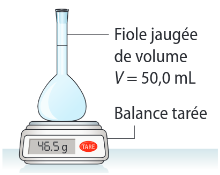
\includegraphics[scale=.6]{Resssources/2GT_DS1_Fig1.png}}\\ \cline{1-4}
	$\theta_f$ (\unit{\celsius}) & \num{-98} & \num{-92} & \num{-71} &\\ \cline{1-4}
	$\theta_{eb}$ (\unit{\celsius}) & \num{57} & \num{102} & \num{149}& \\ \cline{1-4}
	$\rho$ (\unit{\gram\per\milli\liter}) & \num{0,93} & \num{0,88} & \num{0,88}& \\ \cline{1-4}
	\end{tabular}
\end{table}
\begin{enumerate}
	\item Proposer un protocole expérimental permettant d'identifier ces espèces chimiques. \textbf{(1pt)}
\end{enumerate}
\fbox{\begin{minipage}{.9\textwidth}
	\begin{Form}
	\TextField[width = 17cm, height = 5cm,multiline,bordercolor=white]{}
	\end{Form}
	\end{minipage}}
	\fbox{\begin{minipage}{.05\textwidth}
	\vspace{5cm}
	\hspace{.5cm}
	\end{minipage}}
\begin{enumerate}[resume]
	\item Déterminer la masse volumique de l'échantillon suivant. \textbf{(1pt)}
\end{enumerate}
\fbox{\begin{minipage}{.9\textwidth}
	\begin{Form}
	\TextField[width = 17cm, height = 5cm,multiline,bordercolor=white]{}
	\end{Form}
	\end{minipage}}
	\fbox{\begin{minipage}{.05\textwidth}
	\vspace{5cm}
	\hspace{.5cm}
	\end{minipage}}
\begin{enumerate}[resume]
	\item Cette mesure permet-elle d'identifier l'une des espèces ? \textbf{(1pt)}
\end{enumerate}
\fbox{\begin{minipage}{.9\textwidth}
	\begin{Form}
	\TextField[width = 17cm, height = 5cm,multiline,bordercolor=white]{}
	\end{Form}
	\end{minipage}}
	\fbox{\begin{minipage}{.05\textwidth}
	\vspace{5cm}
	\hspace{.5cm}
	\end{minipage}}

\end{document}